%%%%%%%%%%%%%%%%%%%%%%%%%%%%%%%%%%%%%%%%%%%%%%%%%%%%%%%%%%%%%%%%%%%%%%%%%%%%%%%%
%2345678901234567890123456789012345678901234567890123456789012345678901234567890
%        1         2         3         4         5         6         7         8

\documentclass[letterpaper, 10 pt, conference]{ieeeconf}  % Comment this line out if you need a4paper

%\documentclass[a4paper, 10pt, conference]{ieeeconf}      % Use this line for a4 paper

\IEEEoverridecommandlockouts                              % This command is only needed if 
                                                          % you want to use the \thanks command

\overrideIEEEmargins                                      % Needed to meet printer requirements.

%In case you encounter the following error:
%Error 1010 The PDF file may be corrupt (unable to open PDF file) OR
%Error 1000 An error occurred while parsing a contents stream. Unable to analyze the PDF file.
%This is a known problem with pdfLaTeX conversion filter. The file cannot be opened with acrobat reader
%Please use one of the alternatives below to circumvent this error by uncommenting one or the other
%\pdfobjcompresslevel=0
%\pdfminorversion=4

% See the \addtolength command later in the file to balance the column lengths
% on the last page of the document

% The following packages can be found on http:\\www.ctan.org
%\usepackage{graphics} % for pdf, bitmapped graphics files
%\usepackage{epsfig} % for postscript graphics files
%\usepackage{mathptmx} % assumes new font selection scheme installed
%\usepackage{times} % assumes new font selection scheme installed
%\usepackage{amsmath} % assumes amsmath package installed
%\usepackage{amssymb}  % assumes amsmath package installed

\usepackage{graphicx}
\graphicspath{{figures/}}
\usepackage{booktabs}

\usepackage{comment}
\usepackage{xcolor}

\newcommand{\yl}[1]{\commentText{{\color{blue}[\textbf{\textsc{YL}}: \textit{#1}]}}}


\title{\LARGE \bf
Reconfigurable and Scalable Tactile Skin via Braid Kinematics
}
%reconfigurable and scalable tactile sensors using xx structure 

% \author{Gaolin Ge$^{1}$, Donald Luo$^{2}$, Alexander Ching$^{3}$, Shwetak Patel$^{3}$, and Yiyue Luo$^{2}$% <-this % stops a space

\author{Anonymous Authors}

% \thanks{*This work was not supported by any organization}% <-this % stops a space
% \thanks{$^{1}$University of Washington, Mechanical Engineering
%         {\tt\small albert.author@papercept.net}}%
% \thanks{$^{2}$University of Washington, Electrical and Computer Engineering
%         {\tt\small albert.author@papercept.net}}%
% \thanks{$^{3}$University of Washington, Computer Science and Engineering
%         {\tt\small {atching, shwetak} @cs.washington.edu}}%
% }


\begin{document}



\maketitle
\thispagestyle{empty}
\pagestyle{empty}



%%%%%%%%%%%%%%%%%%%%%%%%%%%%%%%%%%%%%%%%%%%%%%%%%%%%%%%%%%%%%%%%%%%%%%%%%%%%%%%%
\begin{abstract}

This electronic document is a ÒliveÓ template. The various components of your paper [title, text, heads, etc.] are already defined on the style sheet, as illustrated by the portions given in this document.

\end{abstract}


%%%%%%%%%%%%%%%%%%%%%%%%%%%%%%%%%%%%%%%%%%%%%%%%%%%%%%%%%%%%%%%%%%%%%%%%%%%%%%%%
\section{INTRODUCTION}

Robotics has advanced greatly in recent years and are now very prevalent in manufacturing with growing instances of direct human interaction. There has been a growing need for robotic systems to be aware of their surroundings so that they can accurately interact with the physical world. Vision based systems, such as optical cameras and lidar, have been very popular for a variety of applications, but for direct tactile sensing they lack the high temporal resolution and dynamic range needed for many scenarios such as fine grain interaction where sensing of direct forces matter. For these situations, robotic skins or wearable sensors provide much better data input. Current solutions are sparse, wired, and cover only part of the limb as well as lack full spatial coverage of an area without custom integrations.


In this work, we propose a reconfigurable sensor integrated skin built around the braid kinematics of McKibben muscles to address this. The braided architecture simultaneously provides mechanical reconfigurability and tactile sensing to a range of conical geometries often found on robot appendages. Our prototype skin conforms to a range of limb sizes with each interlace forming a piezoresistive sensing node. Our research contributions presented in this paper include:

\begin{itemize}
    \item Two Prototpyes and design framework (expand on this, ref design equations)
    \item An empirical characterization of the sensor within the McKibben architecture in various configurations (angles vs pressure)
    \item A companion tool closes the loop between geometry and sensing: it generates the braid structure from the design parameters, computes the braid angle at every node, assigns the angle calibration to each node, and renders live 3D heat maps. 
    \item An evluation of the skin when used on a robotic finger and arm in various real world applications
\end{itemize}


% \begin{itemize}
%   \item Gap: most robotic skins / wearable sensors are sparse, wired, and cover only part of the limb; high-resolution with full-circumference coverage remains hard.
%  \item The key idea is that the sleeve is the sensor: the same braided architecture simultaneously provides mechanical reconfigurability and tactile sensing. Its McKibben-style geometry allows the sleeve to conform and adapt to limbs of different sizes, while every ribbon crossover forms an individual piezoresistive tactile node. Thus, the structure that mechanically conforms the sleeve also defines and distributes its sensing array.
% \end{itemize}

%%%%%%%%%%%%%%%%%%%%%%%%%%%%%%%%%%%%%%%%%%%%%%%%%%%%%%%%%
\section{RELATED WORK}

\begin{figure*}[t]
  \centering
  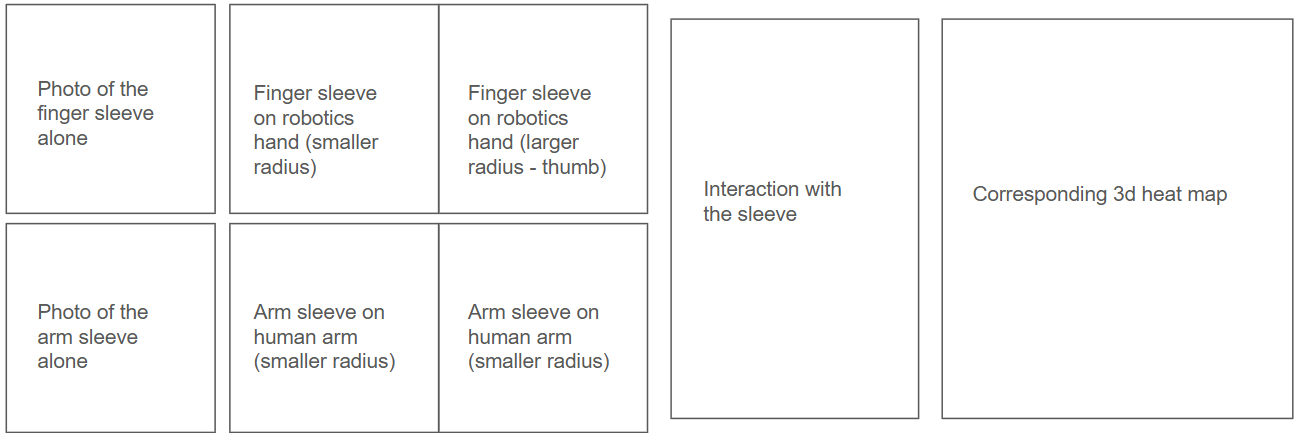
\includegraphics[width=\textwidth]{figures/overview.png}
  \caption{Overview}
  \label{fig:overview}
\end{figure*}

\subsection{Tactile Sensing on Robotics Skins and Smart Textiles}

Tactile sensing for robotic manipulation has advanced rapidly. Vision-based fingertip sensors such as GelSight~\cite{gelsight} can deliver submillimeter spatial resolution. More recent skins scale sensing to larger areas: magnetic patches can be swapped out in seconds~\cite{anyskin}, and stretchable skins wrap robot limbs for physical human-robot interaction~\cite{cushsense}. Together, these works have extended tactile sensing from the fingertip toward the whole limb. Our skin builds on the same sensing principle, but uses a braided geometry rather than a planar row-column sheet to define the node lattice. This distinction is mechanical as well as electrical. In prior textile arrays, the sensing layout is placed onto or integrated into a deformable substrate. In our design, the sensing ribbons themselves form the reconfigurable structure. The same braid therefore determines both how the skin conforms to the limb and where the tactile nodes are located.


In parallel, the HRI community has brought touch sensing onto textiles. Examples include interactive fabrics woven at scale~\cite{jacquard} and touch-sensing cords~\cite{iobraid}. For dense pressure mapping, a common design sandwiches a piezoresistive layer between orthogonal conductive electrodes. The resulting row-column matrix turns each crossover into a pressure sensitive junction~\cite{holm}. This principle has powered fabric-based robot skins~\cite{buscher}, scalable tactile gloves~\cite{tactileglove}, and full-size knitted sensing garments~\cite{tactiletextiles,knits}. These works reach hundreds of sensing points over full garments. Our skin builds on the same principle, using each crossover as a junction. The novelty is that a braided geometry, rather than a row-column sheet, defines the node lattice. As a result, the structure that senses is also the structure that conforms the array to limbs of different sizes.

\subsection{Braided Structures in Robotics and Sensing}

Braided sleeves are well established in robotics. They form the constraining layer of McKibben pneumatic artificial muscles, whose cylindrical braid kinematics couple diameter to length along a characteristic curve~\cite{chou}. Braiding on complex and conical mandrels is likewise mature in composites manufacturing~\cite{braidreview}. Building on this kinematic foundation, we repurpose the braid from an actuator's constraint layer into the body of a tactile sensor.

The braid has also proven valuable as a sensing element in its own right. The Smart Braid approach weaves conductive strands into the muscle sleeve. Contraction can then be estimated from the sleeve's inductance~\cite{smartbraid} and used for closed-loop control of soft actuators~\cite{smartbraidfb}. In HCI, I/O Braid~\cite{iobraid} brings touch sensing to a spiraling textile cord. Inspired by these works, we exploit two further properties of the braid. First, its crossover lattice forms a dense node array for tectile sensing. Second, its diameter-length kinematics, described by the same master curve as a McKibben muscle, predicts how a passive sleeve conforms to limbs of different sizes. These properties let us design one sleeve per limb segment: a cylindrical finger sleeve and a conical forearm sleeve. In both sleeves, every ribbon crossover doubles as a pressure sensitive node, tiling the full circumference of the limb.
%%%%%%%%%%%%%%%%%%%%%%%%%%%%%%%%%%%%%%%%%%%%%%%%%%%%%%%%%%%%%%%%%%%%%%%%%%


\section{METHOD}

\yl{I suggest IIIA Resistive sensing array/braid design: talk about what makes a tactile sensor, why the braiding design makes an array, how it detects pressure. IIIB Reconfigurable mechanical design: talk about your general formulation on symmetrical cylinder and asymmetrical cylinder, no need to mention the particular finger and arm example at this point, you should be describing a general approach first. 
After that, there are two options.
option1: section IIIC Fabrication and assembly: talk about fabrication approach, assembly (keep it general, no need to mention finger or arma in method section, if the fabrication approach is different, mention one is for small scale one is for bigger scale). Section Section IV Tactile sensors for fingers; Section V Tactile sensors for arms. in each section, talk about A sensor design (what you have in IIID), B Characterization, C Visualization.
option2: section IV Fabrication: talk about specific design considerations (what you have in IIID) and fabrication approach for finger and arm specifically. section V Results: characterization, visualization for finger and arm examples }


\begin{figure*}[t]
  \centering
  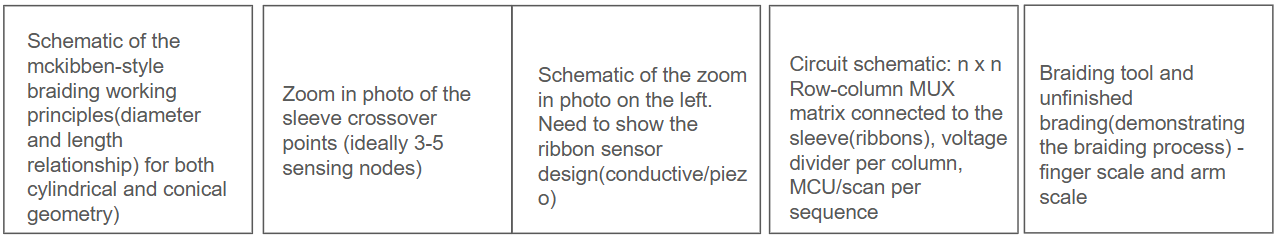
\includegraphics[width=\textwidth]{figures/design and fab.png}
  \caption{design and fab}
  \label{fig:design and fab}
\end{figure*}

\begin{figure*}[t]
  \centering
  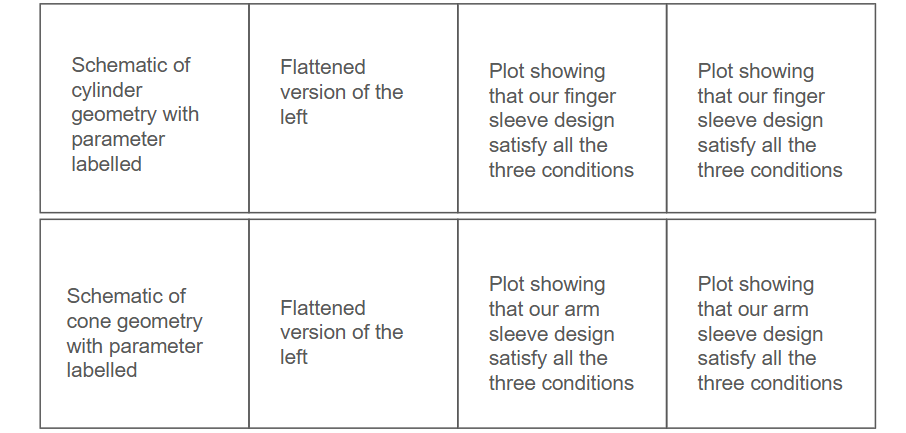
\includegraphics[width=0.8\textwidth]{figures/braiding kinematics.png}
  \caption{braiding kinematics}
  \label{fig:braiding kinematics}
\end{figure*}

\subsection{Resistive Sensing Array and Braid Design}
The key contribution of this work is a reconfigurable tactile sensing skin, and the braided mechanical design of Sec.~III-B is how the skin achieves its reconfigurability. The skin integrates mechanical adaptation and tactile sensing into a single braided structure: each ribbon is a layered stack of a piezoresistive sheet and a conductive fabric layer, and where two ribbons cross, the stackup forms a junction whose resistance drops as the contact pressure rises~\cite{holm}. In readout, each junction sits in a voltage divider, so the pressure at a node appears as a voltage.

Braiding turns this junction principle into a dense array. The skin is a regular braid of $2n$ sensing ribbons, terminated at both ends by collars. Every ribbon crossover forms one sensing node, so a braid with $N$ turns per ribbon contains $2n^2 N$ crossovers that tile the full circumference of the limb. Crossovers that coincide with the collar anchors serve as mechanical pivots and are excluded from readout. The braid geometry itself therefore determines the array layout: as the braid changes diameter and length to conform to the limb, the same sensing ribbons maintain a distributed lattice of pressure sensitive crossovers.

\subsection{Reconfigurable Mechanical Design}\label{sec:braid-layout}
The braid follows McKibben kinematics. As the skin is pulled onto a limb, its diameter and length trade off along a fixed kinematic curve. One skin conforms to a range of limb sizes instead of a single diameter. Collars at both ends fix the ribbon ends and define the usable length. Two geometries cover the limb segments considered in this work: a symmetric segment is modeled as a cylinder, and a tapered segment as a cone.

\subsubsection{Cylinder}
On a cylinder, a braid of ribbon length $b$ with $N$ turns obeys
\begin{equation}
L = b\cos\theta, \qquad N\pi D = b\sin\theta,
\end{equation}
with braid angle $\theta$ measured from the axis and diameter $D$. Eliminating $\theta$ gives the working range as an ellipse arc,
\begin{equation}
\left(\frac{L}{b}\right)^{2} + \left(\frac{D}{D_0}\right)^{2} = 1, \qquad D_0 = \frac{b}{\pi N},
\end{equation}
where $D_0 = b/(\pi N)$ is the jamming diameter, the largest diameter the braid can approach: as the skin expands, the ribbons tilt toward the circumferential direction, and at $D_0$ they would run purely circumferentially. The skin length is therefore a decreasing function of diameter on $[0, D_0)$. Real ribbons have finite width $w$, so neighboring ribbons touch and block further expansion before the braid ever reaches $D_0$; this contact is what we call jamming. Requiring that neighboring ribbons never overlap around the circumference gives a second constraint, $\cos\theta(D) \geq nw/(\pi D)$.

\subsubsection{Cone}
A tapered segment is modeled as a cone of half-angle $\alpha$, and we measure position by the slant distance $s$ from the cone apex. The braid satisfies the master curve
\begin{equation}
b^2 = s_1^2 + s_2^2 - 2 s_1 s_2 \cos N\beta, \qquad \beta = 2\pi\sin\alpha,
\end{equation}
where $s_1$ and $s_2$ are the apex distances of the two ribbon endpoints. Its physical branch is
\begin{equation}
s_2 = s_1\cos N\beta + \sqrt{b^2 - s_1^2\sin^2 N\beta}.
\end{equation}
The Clairaut constant $p = s_1 s_2 \sin(N\beta)/b$ gives the braid angle along the skin, $\theta(s) = \arcsin(p/s)$, which decreases toward the wide end of the cone. On a cone, the skin circumference $2\pi s \sin\alpha$ matches the limb circumference at whatever station the skin sits, so fit along the span is free. What remains is the worn span, the axial length the skin covers on a limb whose entry circumference is $C_1$:
\begin{equation}
\Lambda(C_1) = (s_2 - s_1)\cos\alpha, \qquad s_1 = \frac{C_1/2\pi}{\sin\alpha}.
\end{equation}

\subsection{Fabrication and Assembly}
Ribbons are laser-cut to width and braided on a shaped mandrel. The same process serves both scales in this paper: the small scale skin is braided on a cylindrical mandrel, while the larger tapered skin is braided on a conical mandrel with geodesic guide grooves. After braiding, the ribbon ends are fixed at the collars and the braid is released from the mandrel.




\begin{table}[t]
\centering
\caption{Fabrication parameters for finger sleeve and arm sleeve}
\label{tab:fab}
\resizebox{\columnwidth}{!}{%
\begin{tabular}{lcc}
\toprule
 & Finger (cylinder) & Arm (cone) \\
\midrule
ribbons $2n$ & 20 & 24 \\
turn number $N$ & $1/5$ & $1/3$ \\
ribbon length $b$ & 16~mm & 165~mm \\
ribbon width $w$ & 3~mm & 7~mm \\
cone half-angle $\alpha$ & / & $4.94^\circ$ \\
fabrication angle $\theta_{fab}$ & $33.6^\circ$ & $26.7^\circ$ to $16.3^\circ$ \\
covered diameter & $14.1$ to $22.3$~mm & $44.6$ to $71.1$~mm \\
worn length & $13.3$ to $7.7$~mm & $153.6$ to $140.3$~mm \\
crossovers $2n^2N$ & 40 & 96 \\
sensing nodes & 30 & 96 \\
\bottomrule
\end{tabular}}
\end{table}

%%%%%%%%%%%%%%%%%%%%%%%%%%%%%%%%%%%%%%%%%%%%%%%%%%%%%%%%%%%%%%%%%%%%

\section{FINGER AND ARM SKIN DESIGNS}\label{sec:designs}

\begin{figure}[t]
  \centering
  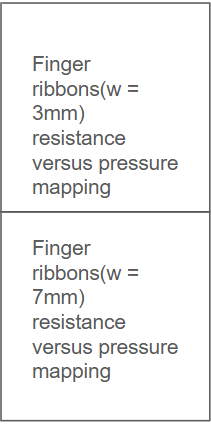
\includegraphics[width=0.6\columnwidth]{figures/RP characterization.png}
  \caption{RP characterization}
  \label{fig:RP characterization}
\end{figure}

The skin described above is a generalized approach rather than a design for one limb: the same braid architecture and the same design equations serve both scales in this paper, a finger skin with 30 sensing nodes and an arm skin with 96. A single skin is expected to fit fingers and forearms across the adult population. Wearable robots typically establish fit by comparing an adjustment range against percentile bounds from anthropometric data~\cite{bluesabino}. We follow the same practice with one difference: the working range of the skin is analytic, so the comparison becomes a proof instead of a lookup table.

\subsection{Finger Skin}
Three published numbers describe the target population. Finger diameters come from the ring-size standard~\cite{iso8653}: US sizes 3 to 13 span inner diameters $D_{min} = 14.1$ to $D_{max} = 22.3$~mm. Segment lengths come from a radiological study of 384 adult hands~\cite{phalanx}: mean phalanx lengths run from 14.88 to 43.63~mm. The binding constraint is the shortest segment, $\ell_{min} = 14.88$~mm, since a sleeve that fits the shortest segment also fits every longer one.

A skin covers the envelope if three conditions hold everywhere on $[D_{min}, D_{max}]$. First, reachability: the braid must open to the largest size, so its jamming diameter satisfies $D_0 \geq D_{max}$. Second, length: the worn length must fit the shortest segment, $L(D) \leq \ell_{min}$. Third, self-jamming: neighboring ribbons must not overlap around the circumference, $\cos\theta(D) \geq nw/(\pi D)$.
The reachability and length conditions give a lower and an upper bound on the ribbon length,
\begin{equation}
\pi N D_{max} \;\leq\; b \;\leq\; \sqrt{\ell_{min}^2 + (\pi N D_{min})^2},
\end{equation}
and a valid ribbon length exists only if the lower bound does not exceed the upper one. Solving this requirement for the turn number gives
\begin{equation}
N \leq \frac{\ell_{min}}{\pi\sqrt{D_{max}^2 - D_{min}^2}},
\end{equation}
which evaluates to $0.274$ for the finger envelope. Based on these conditions, we selected the skin parameters listed in Table~I. Fig.~\ref{} checks the chosen finger design against all three conditions over the full envelope: the worn length stays below the shortest segment everywhere, and the jamming diameter $D_0 = 25.5$~mm lies beyond the largest size; the self-jamming margin stays positive across the envelope. Since the worn length decreases with size and the self-jamming margin is concave in $D$, the endpoint values would certify the full range.

The finger skin follows the process of Sec.~III-C on a cylindrical mandrel, braided at the fabrication angle $\theta_{fab} = 33.6^\circ$ with 3~mm ribbons (Table~I).

\subsection{Arm Skin}
The same argument runs on the cone, with wrist circumference in place of diameter (Fig.~\ref{}). The cone must accept the wrist envelope around the arm, and the worn span must stay useful along the arm: short enough at the smallest wrist to satisfy the anatomy, and long enough at the largest wrist to cover the forearm. The worn span $\Lambda(C_1)$ is decreasing in wrist circumference, so both checks again collapse to endpoints, and the covered range appears in Table~I.

The arm skin follows the process of Sec.~III-C on the conical mandrel with geodesic guide grooves, which set a fabrication angle varying from $26.7^\circ$ to $16.3^\circ$ along the cone (Table~I).


%%%%%%%%%%%%%%%%%%%%%%%%%%%%%%%%%%%%%%%%%%%%%%%%%%%%%%%%


\section{RESULTS}

\begin{figure*}[t]
  \centering
  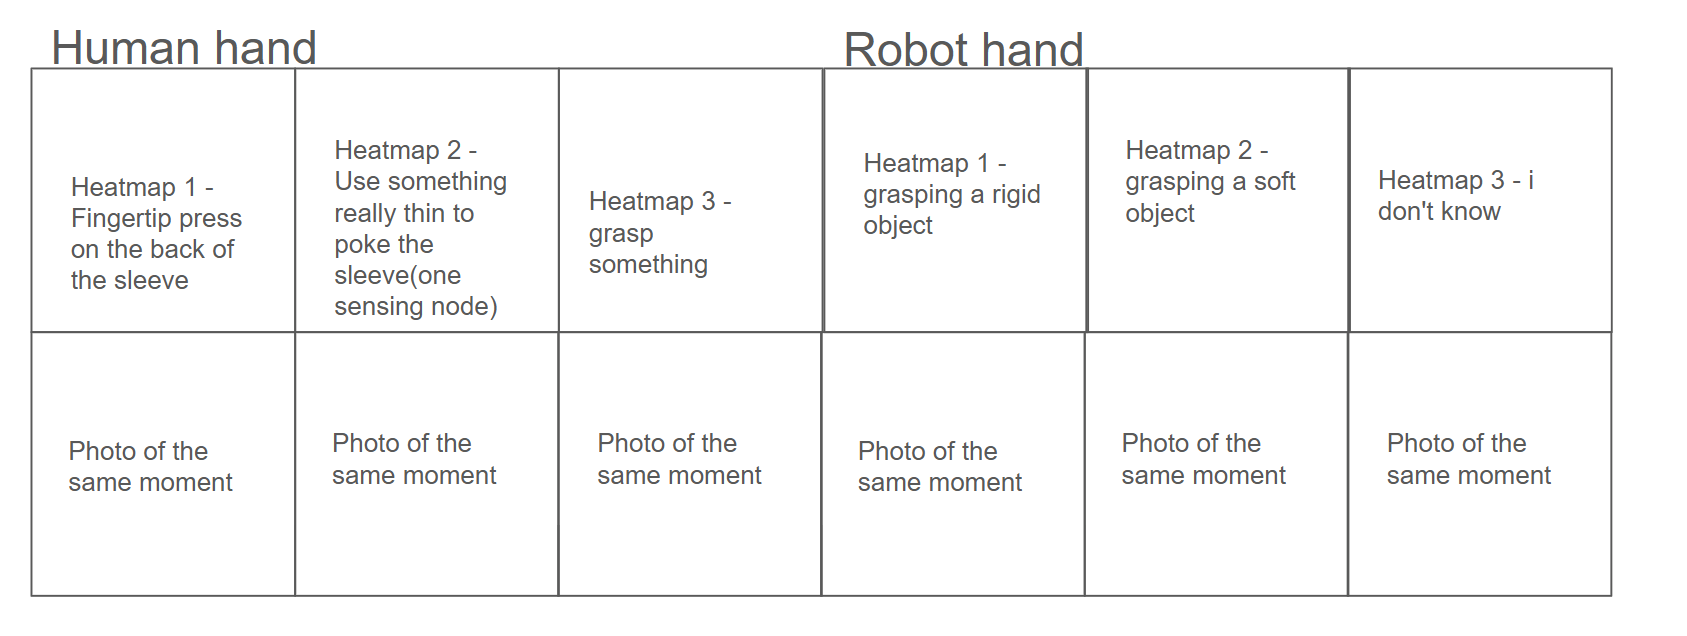
\includegraphics[width=\textwidth]{figures/hand interface.png}
  \caption{hand interface}
  \label{fig:hand interface}
\end{figure*}

\subsection{Pressure versus Resistance across Braid Angles}\label{sec:angle-characterization}
Characterizing the sensing response across braid angles is important because the braid angle changes as the skin adapts to different diameters and lengths. For the conical arm skin, the braid angle also varies along the length of the skin. Since different braid angles produce different resistance baselines, a single pressure-resistance mapping cannot be assumed for all sensing nodes. We therefore characterize the pressure-resistance response at different braid angles to establish the corresponding mappings required for sensing across the skin's reconfigurable geometry.
The braid angle changes the geometry of each ribbon crossover. For two ribbons of width $w$ crossing at braid angle $\theta$, the crossover area is
\begin{equation}
A_{node} = \frac{w^2}{\sin(2\theta)}.
\end{equation}
The crossover area is minimized near $\theta = 45^\circ$ and increases as the braid angle moves away from $45^\circ$. Therefore, changes in braid angle alter the pressure relationship at each sensing node and affect its electrical response.
We characterized this effect for the two ribbon widths used in our prototypes: 3~mm for the finger skin and 7~mm for the arm skin. Both were tested at braid angles of $42^\circ$, $48^\circ$, $52^\circ$, $58^\circ$, $64^\circ$, and $72^\circ$. At each angle, the voltage divider output was recorded as a function of pressure (Fig.~\ref{}).
The measured responses follow the predicted trend, with smaller braid angles producing higher resistance baselines. For the 3~mm ribbons, the response curves remain closely grouped. In contrast, the 7~mm ribbons show a larger variation in baseline resistance across braid angles. This larger variation indicates that a single pressure to resistance mapping is insufficient for all braid configurations. Angle calibration is therefore important for generating accurate real time pressure heat maps, and the tool in Sec.~\ref{sec:tool} assigns these calibrations to individual nodes.

\subsection{Coverage Validation}
measured vs theoretical D-L curve

\subsection{Interactive Design and Visualization Tool}\label{sec:tool}
Two practical needs motivate a companion software tool. First, the braid angle differs from node to node and shifts whenever the sleeve adapts to a different limb size, and Sec.~\ref{sec:angle-characterization} shows that the electrical response depends on this angle. Decoding a worn sleeve therefore requires the current angle at every node. Second, the array wraps a curved surface, so a flat heat map of the node values is difficult to read.

\emph{Geometry generation.} The tool takes the design parameters of Sec.~\ref{sec:designs} as input: target diameter and length, ribbon count, ribbon length, and ribbon width, plus the cone half-angle for tapered limbs. It solves the braid layout of Sec.~\ref{sec:braid-layout} and builds the corresponding three-dimensional ribbon structure.

\emph{Calibration.} Our tool evaluates the braid angle at every node: $\theta = \arcsin(\pi N D / b)$ from the current diameter on the cylinder, and $\theta(s) = \arcsin(p/s)$ node by node along the cone. Each node is assigned the pressure-resistance mapping of the nearest characterized angle from Sec.~\ref{sec:angle-characterization}. 

\emph{3D heat map.} Connected to the readout circuit, the tool renders each calibrated node value as a colored marker at its crossover on the 3D sleeve model. Contact location and intensity are read directly from the 3D sleeve surface instead of being unwrapped from a flat grid. All heat maps in the remainder of this section are rendered by this tool.

\subsection{Hand Interfaces}

plan A

human and robot hand x3 sensors
3 different scenarios, with 3 sensors wearing on different finger parts, all doing same grasping 

1. 3 sensors on the same finger
2. 3 sensors on the proximal joint of fingers
3. 3 sensors on different parts of different fingers


plan B

human and robot hand x1 sensors
9 different scenarios, with 1 sensors wearing on different finger parts/finger, all doing same grasping 

1 sensor on 3 different parts of 3 different fingers (x9 images)

record video 


\subsection{Arm Interfaces}

human arm
ask 3 people to wear, 3 scenarios for each person 

robot arm 
robot arm itself + 2 3d print cases, 3 scenario for each (hand grasping, finger poking, push an object on the arm)

record video

9/12



\begin{figure*}[t]
  \centering
  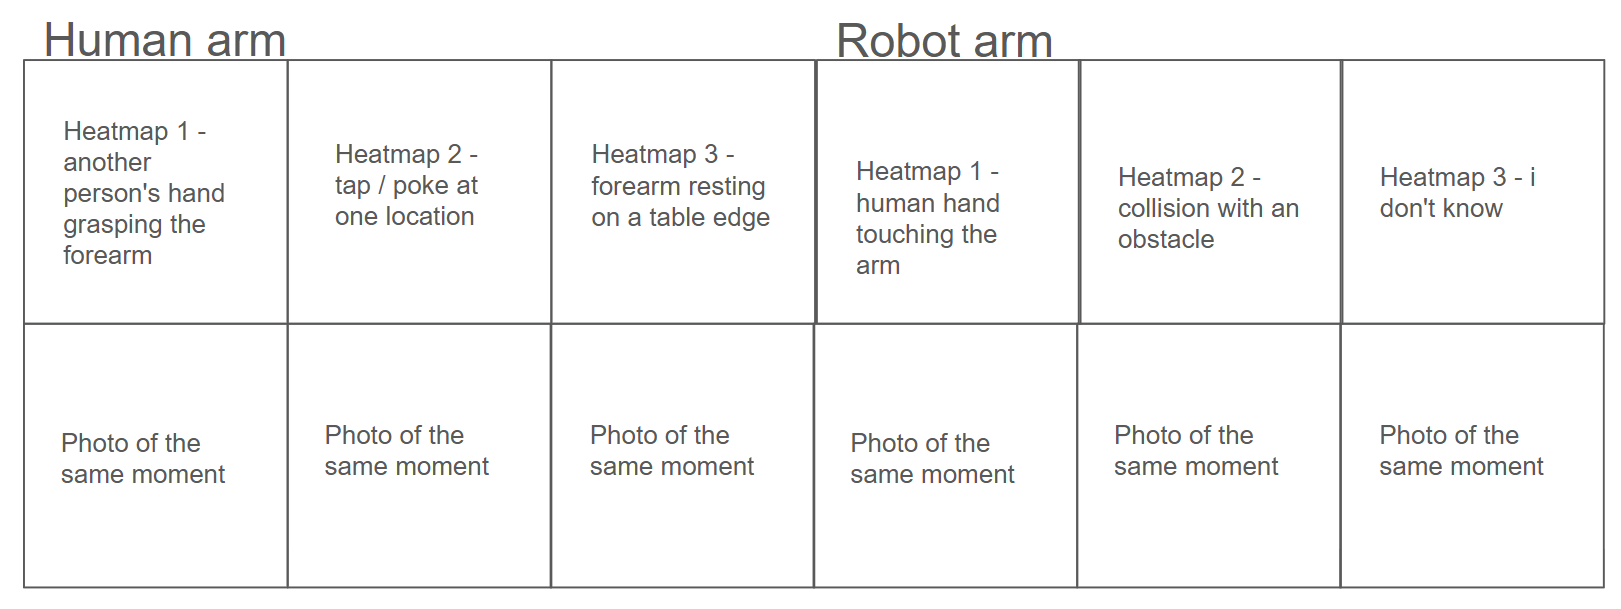
\includegraphics[width=\textwidth]{figures/arm interface.png}
  \caption{Arm Interfaces}
  \label{fig:Arm Interfaces}
\end{figure*}

%%%%%%%%%%%%%%%%%%%%%%%%%%%%%%%%%%%%%%%%%%%%%%%%%%%%%%%%


\section{CONCLUSIONS AND FUTURE WORK}

\addtolength{\textheight}{-12cm}   % This command serves to balance the column lengths
                                  % on the last page of the document manually. It shortens
                                  % the textheight of the last page by a suitable amount.
                                  % This command does not take effect until the next page
                                  % so it should come on the page before the last. Make
                                  % sure that you do not shorten the textheight too much.

%%%%%%%%%%%%%%%%%%%%%%%%%%%%%%%%%%%%%%%%%%%%%%%%%%%%%%%%%%%%%%%%%%%%%%%%%%%%%%%%



%%%%%%%%%%%%%%%%%%%%%%%%%%%%%%%%%%%%%%%%%%%%%%%%%%%%%%%%%%%%%%%%%%%%%%%%%%%%%%%%



%%%%%%%%%%%%%%%%%%%%%%%%%%%%%%%%%%%%%%%%%%%%%%%%%%%%%%%%%%%%%%%%%%%%%%%%%%%%%%%%
\section*{APPENDIX}

Appendixes should appear before the acknowledgment.





%%%%%%%%%%%%%%%%%%%%%%%%%%%%%%%%%%%%%%%%%%%%%%%%%%%%%%%%%%%%%%%%%%%%%%%%%%%%%%%%

References are important to the reader; therefore, each citation must be complete and correct. If at all possible, references should be commonly available publications.



\begin{thebibliography}{99}

\bibitem{gelsight}
W.~Yuan, S.~Dong, and E.~H. Adelson,
``GelSight: High-resolution robot tactile sensors for estimating geometry and force,''
\emph{Sensors}, vol.~17, no.~12, p.~2762, 2017.

\bibitem{anyskin}
R.~Bhirangi, V.~Pattabiraman, E.~Erciyes, Y.~Cao, T.~Hellebrekers, and L.~Pinto,
``AnySkin: Plug-and-play skin sensing for robotic touch,''
in \emph{Proc. IEEE Int. Conf. Robot. Autom. (ICRA)}, 2025, pp.~16563-16570.

\bibitem{cushsense}
B.~Xu, L.~Zhong, G.~Zhang, X.~Liang, D.~Virtue, R.~Madan, and T.~Bhattacharjee,
``CushSense: Soft, stretchable, and comfortable tactile-sensing skin for
physical human-robot interaction,''
in \emph{Proc. IEEE Int. Conf. Robot. Autom. (ICRA)}, 2024, pp.~5694-5701.

\bibitem{jacquard}
I.~Poupyrev, N.-W. Gong, S.~Fukuhara, M.~E. Karagozler, C.~Schwesig, and K.~E. Robinson,
``Project Jacquard: Interactive digital textiles at scale,''
in \emph{Proc. ACM CHI}, 2016, pp.~4216-4227.

\bibitem{iobraid}
S.~Olberding, M.~Wessely, and J.~Steimle,
``I/O Braid: Scalable touch-sensitive lighted cords using spiraling, repeating
sensing textiles and fiber optics,''
in \emph{Proc. ACM UIST}, 2018, pp.~489-502.

\bibitem{holm}
R.~Holm,
\emph{Electric Contacts: Theory and Application}, 4th~ed.\ Berlin: Springer, 1967.

\bibitem{buscher}
G.~H. B\"uscher, R.~K\~oiva, C.~Sch\"urmann, R.~Haschke, and H.~J. Ritter,
``Flexible and stretchable fabric-based tactile sensor,''
\emph{Robot. Auton. Syst.}, vol.~63, pp.~244-252, 2015.

\bibitem{tactileglove}
S.~Sundaram, P.~Kellnhofer, Y.~Li, J.-Y. Zhu, A.~Torralba, and W.~Matusik,
``Learning the signatures of the human grasp using a scalable tactile glove,''
\emph{Nature}, vol.~569, pp.~698-702, 2019.

\bibitem{tactiletextiles}
Y.~Luo, Y.~Li, P.~Sharma, W.~Shou, K.~Wu, M.~Foshey, B.~Li, T.~Palacios,
A.~Torralba, and W.~Matusik,
``Learning human-environment interactions using conformal tactile textiles,''
\emph{Nat. Electron.}, vol.~4, pp.~193-201, 2021.

\bibitem{knits}
I.~Wicaksono, P.~G. Hwang, S.~Droubi, F.~X. Wu, A.~N. Serio, W.~Yan, and J.~A. Paradiso,
``3DKnITS: Three-dimensional digital knitting of intelligent textile sensor for
activity recognition and biomechanical monitoring,''
in \emph{Proc. 44th Annu. Int. Conf. IEEE Eng. Med. Biol. Soc. (EMBC)}, 2022.

\bibitem{chou}
C.-P. Chou and B.~Hannaford,
``Measurement and modeling of McKibben pneumatic artificial muscles,''
\emph{IEEE Trans. Robot. Autom.}, vol.~12, no.~1, pp.~90-102, 1996.

\bibitem{braidreview}
S.~Shang \emph{et al.},
``A comprehensive review on manufacturing large composites with complex
irregular geometry by circular braiding,''
\emph{Int. J. Extreme Manuf.}, 2026, doi:10.1088/2631-7990/ae6bdf.

\bibitem{smartbraid}
W.~Felt, K.~Y. Chin, and C.~D. Remy,
``Contraction sensing with smart braid McKibben muscles,''
\emph{Sensors}, vol.~17, no.~5, p.~1196, 2017.

\bibitem{smartbraidfb}
W.~Felt and C.~D. Remy,
``Smart braid feedback for the closed-loop control of soft robotic systems,''
\emph{Soft Robot.}, vol.~4, no.~3, pp.~261-273, 2017.

\bibitem{bluesabino} C.~K. Bitikofer, S.~Rueda~Parra, R.~Maura, E.~T. Wolbrecht, and J.~C. Perry, ``BLUE SABINO: Development of a BiLateral Upper-Limb Exoskeleton for Simultaneous Assessment of Biomechanical and Neuromuscular Output,'' \emph{Machines}, vol.~12, no.~9, Art.~617, 2024.

\bibitem{iso8653} \emph{Jewellery: Ring-sizes. Definition, Measurement and Designation}, ISO 8653:2016, International Organization for Standardization, Geneva, 2016.

\bibitem{phalanx} A.~R.~B. Santoso, E.~Mustamsir, and T.~E.~C.~J. Huwae, ``Radiological analysis of finger length ratio and dimensional profile of finger anatomy morphology,'' \emph{Journal of Medical Science and Research}, 2026. [Online]. Available: \url{https://journalmsr.com/radiological-analysis-of-finger-length-ratio-and-dimensional-profile-of-finger-anatomy-morphology/}



\end{thebibliography}




\end{document}
